% !TeX program = xelatex
\documentclass[a4paper,10pt]{article}

% ============================================================================
% សន្លឹកកិច្ចការសិស្ស ស-ខ្មៅ (Student Guided-Inquiry Worksheet - Grade 8 15.1 CIRC1)
% បរិបទ៖ គ្មានស្លាយ LCD — សិស្សវាស់ គូស និងបំពេញដោយផ្ទាល់លើសន្លឹកកិច្ចការ (មិនបាច់កាត់បិទ)
% វិធីសាស្ត្រ៖ Contrasting Cases & Variation-Theory Locus Inquiry + Faded Proof
% ============================================================================
\usepackage[a4paper, left=1.0cm, right=1.0cm, top=0.80cm, bottom=1.00cm, footskip=0.50cm]{geometry}
\usepackage{amsmath, amssymb}
\usepackage{unicode-math}
\usepackage{fontspec}
\usepackage{array, colortbl}
\usepackage[table]{xcolor}
\usepackage{enumitem}
\usepackage{pifont}
\usepackage{fancyhdr}
\usepackage{lastpage}
\usepackage{tikz}
\usepackage[most]{tcolorbox}
\usetikzlibrary{calc, arrows.meta, angles, quotes, decorations.markings, positioning, babel}

\makeatletter
\let\@expl@@@mark@update@singlecol@structures@@\relax
\makeatother

\providecommand{\NGSFindFonts}{%
  \IfFileExists{C:/Windows/Fonts/cambria.ttc}{%
    \def\NGSSysPath{C:/Windows/Fonts/}%
    \def\NGSUserPath{C:/Users/KIT/AppData/Local/Microsoft/Windows/Fonts/}%
  }{%
    \IfFileExists{./fonts/KhmerOSsiemreap.ttf}{\def\NGSSysPath{./fonts/}\def\NGSUserPath{./fonts/}}{%
    \IfFileExists{../fonts/KhmerOSsiemreap.ttf}{\def\NGSSysPath{../fonts/}\def\NGSUserPath{../fonts/}}{%
    \IfFileExists{../../fonts/KhmerOSsiemreap.ttf}{\def\NGSSysPath{../../fonts/}\def\NGSUserPath{../../fonts/}}{%
    \IfFileExists{../../../fonts/KhmerOSsiemreap.ttf}{\def\NGSSysPath{../../../fonts/}\def\NGSUserPath{../../../fonts/}}{%
    \IfFileExists{../../../../fonts/KhmerOSsiemreap.ttf}{\def\NGSSysPath{../../../../fonts/}\def\NGSUserPath{../../../../fonts/}}{%
    \IfFileExists{../../../../../fonts/KhmerOSsiemreap.ttf}{\def\NGSSysPath{../../../../../fonts/}\def\NGSUserPath{../../../../../fonts/}}{%
    \IfFileExists{../../../../../../fonts/KhmerOSsiemreap.ttf}{\def\NGSSysPath{../../../../../../fonts/}\def\NGSUserPath{../../../../../../fonts/}}{%
      \def\NGSSysPath{../../../../../../../fonts/}\def\NGSUserPath{../../../../../../../fonts/}%
    }}}}}}}%
  }%
}
\NGSFindFonts

\setmathfont[Path={\NGSSysPath}, FontIndex=1, Scale=1.02]{cambria.ttc}
\defaultfontfeatures{Ligatures=TeX}

\setmainfont[
  Path={\NGSUserPath}, Extension=.ttf, Script=Khmer,
  BoldFont={KhmerOSsiemreap}, BoldFeatures={FakeBold=1.8},
  ItalicFont={KhmerOSsiemreap}, ItalicFeatures={FakeSlant=0.25},
  BoldItalicFont={KhmerOSsiemreap}, BoldItalicFeatures={FakeBold=1.8, FakeSlant=0.25}
]{KhmerOSsiemreap}

\newfontfamily\muol[Path={\NGSUserPath}, Extension=.ttf, Script=Khmer]{KhmerOSmuollight}
\newfontfamily\TimesEn[Path={\NGSSysPath}, Extension=.ttf, BoldFont={timesbd}, ItalicFont={timesi}, BoldItalicFont={timesbi}]{times}
\newfontfamily\CalibriFont[Path={\NGSSysPath}, Extension=.ttf]{calibri}
\newfontfamily\Tacteing[Path={\NGSUserPath}]{TACTENG.TTF}

\XeTeXlinebreaklocale "km"
\XeTeXlinebreakskip = 0pt plus 1pt minus 0.1pt

\definecolor{panelgray}{gray}{0.93}
\definecolor{headgray}{gray}{0.85}

\pagestyle{fancy}
\fancyhf{}
\renewcommand{\headrulewidth}{0pt}
\fancyfoot[L]{\fontsize{8.0pt}{10pt}\selectfont អនុវិទ្យាល័យព្រះក្រសាំង \en{|} គណិតវិទ្យា ថ្នាក់ទី៨ \en{---} មេរៀនទី១៥ (១. សញ្ញាណនិងការកំណត់រង្វង់) \en{|} គ្រូបង្រៀន៖ ហុក ប៊ុនថែន}
\fancyfoot[R]{\fontsize{8.2pt}{10pt}\selectfont ទំព័រ \en{\thepage\ / \pageref{LastPage}}}

\setlength{\parindent}{0pt}
\setlength{\parskip}{0pt}
\setlength{\tabcolsep}{4pt}

\newcommand{\en}[1]{{\TimesEn #1}}
\newcommand{\enbf}[1]{{\TimesEn\bfseries #1}}
\newcommand{\unit}[1]{\,\text{\en{#1}}}
\newcommand{\cnum}[1]{\mbox{\fontsize{10pt}{12pt}\selectfont\ding{\numexpr181+#1\relax}}}
\newcommand{\chkbox}{\tikz[baseline=-0.15ex]\draw[black, line width=0.85pt] (0,0) rectangle (0.24cm,0.24cm);}
\newcommand{\tri}[1]{\ensuremath{\triangle #1}}
\newcommand{\ang}[1]{\ensuremath{\angle #1}}
\newcommand{\blank}[1]{\underline{\hspace{#1}}}

\newcommand{\secbox}[2]{%
  \begin{tcolorbox}[
    enhanced, sharp corners, colback=headgray, colframe=black,
    boxrule=0.95pt, boxsep=1pt, top=2.0pt, bottom=2.0pt, left=6pt, right=6pt,
    before skip=3pt, after skip=2pt
  ]
    {\muol\fontsize{9.2pt}{13.2pt}\selectfont #1}\hfill{\fontsize{8.2pt}{11.5pt}\selectfont\textbf{#2}}
  \end{tcolorbox}%
}

\newcolumntype{L}[1]{>{\raggedright\arraybackslash}p{#1}}
\newcolumntype{C}[1]{>{\centering\arraybackslash}p{#1}}

\tikzset{
  tk1/.style={postaction={decorate},decoration={markings,mark=at position 0.50 with {\draw[black, line width=1.0pt] (0,-0.10)--(0,0.10);}}},
  tk2/.style={postaction={decorate},decoration={markings,
    mark=at position 0.44 with {\draw[black, line width=1.0pt] (0,-0.10)--(0,0.10);},
    mark=at position 0.56 with {\draw[black, line width=1.0pt] (0,-0.10)--(0,0.10);}}}
}

\newcommand{\rightbox}[4][0.18]{%
  \draw[black, line width=0.8pt]
    ($(#3)!#1!(#2)$) -- ($($(#3)!#1!(#2)$)+($(#3)!#1!(#4)$)-(#3)$) -- ($(#3)!#1!(#4)$);
}

\begin{document}
\fontsize{9.1pt}{13.3pt}\selectfont

% ============================================================================
% ទំព័រទី ១៖ E1 + E2 ករណីប្រៀបធៀបទាំង ៤ (Contrasting Cases) + E3 ទ្រឹស្ដីបទ & ធនាគារហេតុផល
% ============================================================================
\begin{tcolorbox}[
  enhanced, sharp corners, colback=white, colframe=black,
  boxrule=1.1pt, boxsep=1.5pt, top=3pt, bottom=3pt, left=6pt, right=6pt
]
  \noindent
  \begin{minipage}[c]{12.2cm}
    {\muol\fontsize{10.3pt}{14.5pt}\selectfont សន្លឹកកិច្ចការសិស្ស ១៥.១ ៖ សញ្ញាណ និងការកំណត់រង្វង់}\\[1.5pt]
    \fontsize{8.5pt}{11.8pt}\selectfont
    \textbf{ឈ្មោះសិស្ស៖} \blank{4.2cm} \quad \textbf{ក្រុមទី៖} \blank{1.2cm} \quad \textbf{ថ្នាក់ទី៨៖} \blank{1.0cm}\\[1.5pt]
    \textbf{បេសកកម្ម E1 (អណ្ដូងទឹកភូមិ ៣)៖} ទាយជាមុន៖ (ក) ភូមិ ៣ មិនរត់ត្រង់ជួរ មានអណ្ដូងស្មើចម្ងាយ \blank{1.1cm} កន្លែង \en{|} (ខ) រត់ត្រង់ជួរ៖ \blank{1.1cm} កន្លែង
  \end{minipage}%
  \hfill
  \begin{minipage}[c]{6.1cm}
    \centering
    {\fontsize{7.5pt}{9.5pt}\selectfont\textbf{បន្ទះផ្ទៀងខ្នាតពិត \en{5.00 cm} (\en{Print 100\%})}}\\[1pt]
    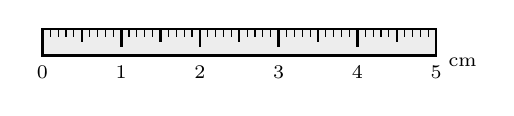
\begin{tikzpicture}[x=1cm, y=1cm, every node/.style={font=\scriptsize, text=black}]
      \draw[black, line width=1.0pt, fill=panelgray] (0,0) rectangle (5.0, 0.34);
      \foreach \m in {0,...,50}{\draw[black, line width=0.4pt] (\m*0.1,0.34)--(\m*0.1,0.24);}
      \foreach \h in {0,0.5,...,5.0}{\draw[black, line width=0.75pt] (\h,0.34)--(\h,0.18);}
      \foreach \c in {0,1,2,3,4,5}{
        \draw[black, line width=1.0pt] (\c,0.34)--(\c,0.11);
        \node[below=0.5pt, font=\scriptsize] at (\c, 0.02) {\en{\c}};
      }
      \node[right=1pt, font=\scriptsize] at (5.0,-0.08) {\en{cm}};
    \end{tikzpicture}
  \end{minipage}
\end{tcolorbox}

\secbox{ផ្នែក ក \enbf{(E2 Explore)} ៖ ការរកឃើញតាមករណីប្រៀបធៀបទាំង \enbf{4 (Contrasting Cases)}}{១១ នាទី \en{---} ប្រើបន្ទាត់ កែង និងដែកឈាន}

\noindent\textbf{ការណែនាំ៖} ប្រើបន្ទាត់ កែង និងដែកឈាន គូសរកផ្ចិតរង្វង់ក្នុងប្រអប់ខ្នាតពិតទាំង ៤ ខាងក្រោម រួចបំពេញតារាងសំយោគ៖

\vspace{2pt}
\noindent
\begin{minipage}[t]{9.30cm}
  \begin{tcolorbox}[enhanced, sharp corners, colback=white, colframe=black, boxrule=0.85pt, boxsep=1pt, top=1.5pt, bottom=1.5pt, left=4pt, right=4pt]
    \textbf{ករណីទី ១ ៖ ចំណុច $A$ តែមួយគត់}\\[0.5pt]
    {\fontsize{8.1pt}{11.0pt}\selectfont យកចំណុច $O_1, O_2$ និងដៅ $O_3$ ខ្លួនឯង ជាផ្ចិត រួចគូសរង្វង់កាត់តាម $A$ ៖}\\[1pt]
    \begin{center}
    \begin{tikzpicture}[x=1cm, y=1cm, every node/.style={font=\footnotesize, text=black}]
      \draw[gray!45, dashed] (0,0) rectangle (8.3, 2.45);
      \coordinate (A) at (4.15, 1.32);
      \coordinate (O1) at (3.30, 1.32);
      \coordinate (O2) at (4.90, 0.90);
      \draw[black, line width=0.8pt, densely dotted] (O1) circle (0.85);
      \fill[black] (A) circle (1.5pt) node[right=2pt] {$A$};
      \fill[black] (O1) circle (1.3pt) node[left=2pt] {$O_1$};
      \fill[black] (O2) circle (1.3pt) node[below right=1pt] {$O_2$};
      \node[anchor=south west, font=\scriptsize] at (0.10,0.05) {គូសរង្វង់ផ្ចិត $O_2$ កាត់ $A$ និងដៅ $O_3$ មួយទៀត!};
    \end{tikzpicture}
    \end{center}
  \end{tcolorbox}
\end{minipage}%
\hfill
\begin{minipage}[t]{9.30cm}
  \begin{tcolorbox}[enhanced, sharp corners, colback=white, colframe=black, boxrule=0.85pt, boxsep=1pt, top=1.5pt, bottom=1.5pt, left=4pt, right=4pt]
    \textbf{ករណីទី ២ ៖ ចំណុចពីរ $A$ និង $B$ ($AB = 3.00\unit{cm}$)}\\[0.5pt]
    {\fontsize{8.1pt}{11.0pt}\selectfont សង់មេដ្យាទ័រ $\Delta$ នៃ $AB$ ត្រង់ចំណុចកណ្ដាល $I$ រួចគូសរង្វង់ផ្ចិតលើ $\Delta$ ៖}\\[1pt]
    \begin{center}
    \begin{tikzpicture}[x=1cm, y=1cm, every node/.style={font=\footnotesize, text=black}]
      \draw[gray!45, dashed] (0,0) rectangle (8.3, 2.45);
      \coordinate (A) at (2.65, 1.25);
      \coordinate (B) at (5.65, 1.25);
      \coordinate (I) at (4.15, 1.25);
      \draw[black, line width=1.1pt] (A) -- (B);
      \draw[black, line width=0.75pt, densely dashed] (4.15, 0.52) -- (4.15, 2.32) node[right=2pt] {$\Delta$};
      \rightbox[0.18]{4.15,2.32}{I}{B}
      \fill[black] (A) circle (1.5pt) node[left=2pt] {$A$};
      \fill[black] (B) circle (1.5pt) node[right=2pt] {$B$};
      \fill[black] (I) circle (1.3pt) node[below right=1pt] {$I$};
      \fill[black] (4.15, 1.92) circle (1.3pt) node[left=2pt] {$O_1$};
      \node[anchor=south west, font=\scriptsize] at (0.10,0.05) {វាស់ផ្ទៀង៖ $O_1A = \blank{0.9cm}\unit{cm}$, $O_1B = \blank{0.9cm}\unit{cm}$};
    \end{tikzpicture}
    \end{center}
  \end{tcolorbox}
\end{minipage}

\vspace{2pt}
\noindent
\begin{minipage}[t]{9.30cm}
  \begin{tcolorbox}[enhanced, sharp corners, colback=white, colframe=black, boxrule=0.85pt, boxsep=1pt, top=1.5pt, bottom=1.5pt, left=4pt, right=4pt]
    \textbf{ករណីទី ៣ ៖ បីចំណុច $A, B, C$ មិនស្ថិតលើបន្ទាត់តែមួយ}\\[0.5pt]
    {\fontsize{8.1pt}{11.0pt}\selectfont គូសបន្តមេដ្យាទ័រ $\Delta_1$ (នៃ $AB$) និង $\Delta_2$ (នៃ $AC$) រកប្រសព្វ $O$ រួចគូសរង្វង់៖}\\[1pt]
    \begin{center}
    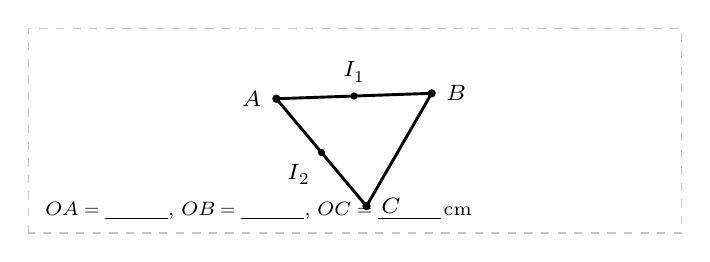
\begin{tikzpicture}[x=1cm, y=1cm, every node/.style={font=\footnotesize, text=black}]
      \draw[gray!45, dashed] (0,0) rectangle (8.3, 2.60);
      \coordinate (O) at (4.15, 1.38);
      \coordinate (A) at ($(O)+(162:1.05)$);
      \coordinate (B) at ($(O)+(22:1.05)$);
      \coordinate (C) at ($(O)+(-82:1.05)$);
      \coordinate (Iab) at ($(A)!0.5!(B)$);
      \coordinate (Iac) at ($(A)!0.5!(C)$);
      \draw[black, line width=1.05pt] (A) -- (B) -- (C) -- cycle;
      \fill[black] (A) circle (1.5pt) node[left=2pt] {$A$};
      \fill[black] (B) circle (1.5pt) node[right=2pt] {$B$};
      \fill[black] (C) circle (1.5pt) node[right=2pt] {$C$};
      \fill[black] (Iab) circle (1.3pt) node[above=1.5pt] {$I_1$};
      \fill[black] (Iac) circle (1.3pt) node[below left=1pt] {$I_2$};
      \node[anchor=south west, font=\scriptsize] at (0.10,0.05) {$OA=\blank{0.8cm}$, $OB=\blank{0.8cm}$, $OC=\blank{0.8cm}\unit{cm}$};
    \end{tikzpicture}
    \end{center}
  \end{tcolorbox}
\end{minipage}%
\hfill
\begin{minipage}[t]{9.30cm}
  \begin{tcolorbox}[enhanced, sharp corners, colback=white, colframe=black, boxrule=0.85pt, boxsep=1pt, top=1.5pt, bottom=1.5pt, left=4pt, right=4pt]
    \textbf{ករណីទី ៤ (អន្ទាក់) ៖ បីចំណុច $A, B, C$ រត់ត្រង់ជួរ}\\[0.5pt]
    {\fontsize{8.1pt}{11.0pt}\selectfont សង់មេដ្យាទ័រ $\Delta_1 \perp AB$ និង $\Delta_2 \perp BC$ ហើយសង្កេតទីតាំង $\Delta_1, \Delta_2$ ៖}\\[1pt]
    \begin{center}
    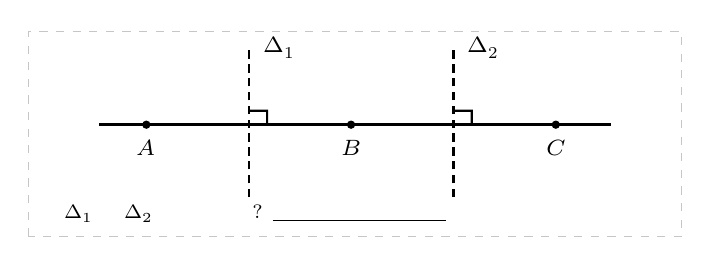
\begin{tikzpicture}[x=1cm, y=1cm, every node/.style={font=\footnotesize, text=black}]
      \draw[gray!45, dashed] (0,0) rectangle (8.3, 2.60);
      \draw[black, line width=1.1pt] (0.9, 1.42) -- (7.4, 1.42);
      \coordinate (A) at (1.5, 1.42);
      \coordinate (B) at (4.1, 1.42);
      \coordinate (C) at (6.7, 1.42);
      \coordinate (M1) at (2.8, 1.42);
      \coordinate (M2) at (5.4, 1.42);
      \draw[black, line width=0.85pt, densely dashed] (2.8, 0.50) -- (2.8, 2.40) node[right=1.5pt] {$\Delta_1$};
      \draw[black, line width=0.85pt, densely dashed] (5.4, 0.50) -- (5.4, 2.40) node[right=1.5pt] {$\Delta_2$};
      \rightbox[0.18]{2.8,2.40}{M1}{B}
      \rightbox[0.18]{5.4,2.40}{M2}{C}
      \fill[black] (A) circle (1.5pt) node[below=2pt] {$A$};
      \fill[black] (B) circle (1.5pt) node[below=2pt] {$B$};
      \fill[black] (C) circle (1.5pt) node[below=2pt] {$C$};
      \node[anchor=south west, font=\scriptsize] at (0.10,0.05) {តើ $\Delta_1$ និង $\Delta_2$ កាត់គ្នាឬស្របគ្នា? \blank{2.2cm}};
    \end{tikzpicture}
    \end{center}
  \end{tcolorbox}
\end{minipage}

\vspace{2.5pt}
{\renewcommand{\arraystretch}{1.18}
\noindent\begin{tabular}{|L{4.3cm}|C{3.8cm}|L{5.6cm}|C{4.3cm}|}
\hline
\rowcolor{headgray}\textbf{ករណីប្រៀបធៀប} & \textbf{ទីតាំងចំណុចដែលឱ្យ} & \textbf{សំណុំទីតាំងផ្ចិតរង្វង់ $O$} & \textbf{ចំនួនរង្វង់ដែលគូសបាន} \\
\hline
ករណីទី ១ & ចំណុច $A$ តែ ១ & គ្រប់ចំណុចក្នុងប្លង់ (ក្រៅពី $A$) & \blank{2.8cm} \\
\hline
ករណីទី ២ & ពីរចំណុច $A$ និង $B$ & នៅលើ \blank{3.6cm} នៃ $AB$ & \blank{2.8cm} \\
\hline
ករណីទី ៣ & $A, B, C$ មិនរត់ត្រង់ជួរ & ចំណុចប្រសព្វ \blank{2.5cm} នៃមេដ្យាទ័រ & \blank{2.8cm} \\
\hline
ករណីទី ៤ (អន្ទាក់) & $A, B, C$ រត់ត្រង់ជួរ & $\Delta_1 \parallel \Delta_2$ (\blank{2.8cm} ប្រសព្វ) & \blank{2.8cm} \\
\hline
\end{tabular}}

\secbox{ផ្នែក ខ \enbf{(E3 Explain)} ៖ សង្ខេបនិយមន័យ ទ្រឹស្ដីបទ និងធនាគារហេតុផល \enbf{1--5}}{៦ នាទី \en{---} បំពេញនិងទុកប្រើក្នុងសម្រាយ}

\noindent
\begin{minipage}[t]{9.6cm}
  \fontsize{8.9pt}{12.8pt}\selectfont
  \textbf{១. បំពេញនិយមន័យ និងទ្រឹស្ដីបទ (សៀវភៅគោល ទំ.១៩៧--១៩៨)៖}\\[1.5pt]
  $\bullet$ រង្វង់ផ្ចិត $O$ កាំ $r$ កំណត់សរសេរដោយ \blank{1.5cm} គឺជាសំណុំគ្រប់ចំណុច $M$ ដែល $OM =$ \blank{1.0cm} ។\\[1.5pt]
  $\bullet$ អង្កត់ភ្ជាប់ពីរចំណុចលើរង្វង់ហៅថា \blank{2.2cm} ។ បើវាកាត់តាមផ្ចិត $O$ ហៅថា \blank{2.2cm} ដែលមានប្រវែង $d =$ \blank{1.1cm} ។\\[1.5pt]
  $\bullet$ \textbf{ទ្រឹស្ដីបទ៖} តាមបីចំណុចដែល\textbf{មិនស្ថិតលើបន្ទាត់តែមួយ} គេអាចគូសបានរង្វង់ \blank{2.1cm} ដែលកាត់តាមចំណុចទាំងបីនោះ ។
\end{minipage}%
\hfill
\begin{minipage}[t]{9.0cm}
  \begin{tcolorbox}[enhanced, sharp corners, colback=panelgray, colframe=black, boxrule=0.85pt, boxsep=1pt, top=2.5pt, bottom=2.5pt, left=5pt, right=5pt]
    {\muol\fontsize{8.7pt}{12.0pt}\selectfont ធនាគារហេតុផល \enbf{(Warrant Bank)} សម្រាប់យោង៖}\\[1.5pt]
    \fontsize{8.3pt}{11.6pt}\selectfont
    \cnum{1} \textbf{និយមន័យរង្វង់ $C(O,r)$៖} $OA=OB=OC=r \Rightarrow A,B,C \in C(O,r)$\\
    \cnum{2} \textbf{លក្ខណៈមេដ្យាទ័រ៖} $O$ នៅលើមេដ្យាទ័រនៃអង្កត់ $XY \iff OX = OY$\\
    \cnum{3} \textbf{លក្ខណៈឆ្លង៖} បើ $OA=OC$ និង $OA=OB$ នោះ $OA=OB=OC$\\
    \cnum{4} \textbf{ទ្រឹស្ដីបទការកំណត់រង្វង់៖} ៣ ចំណុចមិនរត់ត្រង់ជួរ កំណត់រង្វង់តែ ១ គត់\\
    \cnum{5} \textbf{បន្ទាត់ស្រប៖} បន្ទាត់ពីរកែងនឹងបន្ទាត់តែមួយ ជាបន្ទាត់ស្របគ្នា ($\Delta_1\parallel\Delta_2$)
  \end{tcolorbox}
\end{minipage}

\newpage

% ============================================================================
% ទំព័រទី ២៖ E4 សម្រាយបញ្ជាក់បន្ថយជំនួយ + E5 ប្រតិបត្តិខ្នាតពិត AB=6 cm + Exit Check & កិច្ចការផ្ទះ
% ============================================================================
\secbox{ផ្នែក គ \enbf{(E4 Elaborate)} ៖ លំហាត់គំរូ (ទំ.១៩៨) — សម្រាយបញ្ជាក់តាមតារាងហេតុផល}{១០ នាទី \en{---} គូស [tracing] និងបំពេញហេតុផល}

\noindent
\begin{minipage}[c]{5.25cm}
  \centering
  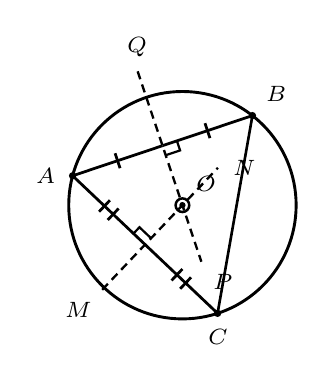
\begin{tikzpicture}[scale=0.95, every node/.style={font=\footnotesize, text=black}]
    \coordinate (O) at (0,0);
    \pgfmathsetmacro{\R}{1.52}
    \coordinate (A) at (165:\R);
    \coordinate (B) at (52:\R);
    \coordinate (C) at (-72:\R);
    \coordinate (Iac) at ($(A)!0.5!(C)$);
    \coordinate (Iab) at ($(A)!0.5!(B)$);
    \draw[black, line width=1.05pt] (O) circle (\R);
    \draw[black, line width=1.0pt, tk1] (A) -- (Iab);
    \draw[black, line width=1.0pt, tk1] (Iab) -- (B);
    \draw[black, line width=1.0pt, tk2] (A) -- (Iac);
    \draw[black, line width=1.0pt, tk2] (Iac) -- (C);
    \draw[black, line width=0.95pt] (B) -- (C);
    \draw[black, line width=0.85pt, densely dashed] ($(O)!2.15!(Iac)$) node[below left=1pt] {$M$} -- ($(O)!-0.95!(Iac)$) node[right=2pt] {$N$};
    \draw[black, line width=0.85pt, densely dashed] ($(O)!2.25!(Iab)$) node[above=1.5pt] {$Q$} -- ($(O)!-0.95!(Iab)$) node[below right=1pt] {$P$};
    \rightbox[0.16]{A}{Iac}{O}
    \rightbox[0.16]{B}{Iab}{O}
    \fill[black] (A) circle (1.4pt) node[left=2.5pt] {$A$};
    \fill[black] (B) circle (1.4pt) node[above right=2pt] {$B$};
    \fill[black] (C) circle (1.4pt) node[below=2pt] {$C$};
    \draw[black, line width=0.9pt] (O) circle (2.6pt);
    \fill[black] (O) circle (1.2pt) node[above right=2pt] {$O$};
  \end{tikzpicture}
\end{minipage}%
\hfill
\begin{minipage}[c]{13.45cm}
  \textbf{ប្រធាន៖} គេមានបីចំណុច $A, B, C$ មិនស្ថិតលើបន្ទាត់តែមួយ ។ តាង $MN$ ជាមេដ្យាទ័រនៃ $AC$ និង $PQ$ ជាមេដ្យាទ័រនៃ $AB$ ដែលប្រសព្វគ្នាត្រង់ $O$ ។ ស្រាយបញ្ជាក់ថា $A, B, C$ ស្ថិតលើរង្វង់តែមួយ ។\\[3pt]
  {\renewcommand{\arraystretch}{1.36}
  \begin{tabular}{|C{1.1cm}|L{8.3cm}|L{3.25cm}|}
    \hline
    \rowcolor{headgray}\textbf{ជំហាន} & \textbf{អំណះអំណាងសម្រាយបញ្ជាក់ (បំពេញចន្លោះ)} & \textbf{លេខហេតុផល (\cnum{1}--\cnum{5})} \\
    \hline
    ១ & ដោយ $O$ ស្ថិតលើមេដ្យាទ័រ $MN$ នៃអង្កត់ $AC$ គេបាន $OA =$ \blank{1.3cm} & តាម \cnum{2} \\
    \hline
    ២ & ដោយ $O$ ស្ថិតលើមេដ្យាទ័រ $PQ$ នៃអង្កត់ $AB$ គេបាន $OA =$ \blank{1.3cm} & តាម \blank{1.4cm} \\
    \hline
    ៣ & តាមជំហាន ១ និង ២ គេទាញបាន $OA =$ \blank{1.1cm} $=$ \blank{1.1cm} & តាម \blank{1.4cm} \\
    \hline
    ៤ & ដូចនេះរង្វង់ផ្ចិត \blank{0.8cm} កាំ $r = OA$ កាត់តាមចំណុច \blank{1.8cm} តែមួយគត់ & តាម \blank{1.4cm} \\
    \hline
  \end{tabular}}\\[4pt]
  {\fontsize{8.7pt}{13pt}\selectfont\textbf{សំណួរត្រិះរិះ (\en{EIA 30s})៖} ហេតុអ្វីបានជាមេដ្យាទ័រទី៣ នៃជ្រុង $BC$ ក៏ត្រូវតែកាត់តាមចំណុច $O$ ដែរ?\\[2pt]
  ចម្លើយ៖ \blank{11.6cm}}
\end{minipage}

\vspace{3pt}
\secbox{ផ្នែក ឃ \enbf{(E5 Practice)} ៖ លំហាត់ប្រតិបត្តិ (ទំ.១៩៨) — ពិសោធន៍រង្វង់ពីរលើអង្កត់ខ្នាតពិត \enbf{AB = 6.00 cm}}{៦.៥ នាទី \en{---} គូសធ្នូរង្វង់ប្រសព្វដោយដែកឈានលើខ្នាតពិត 1:1}

\noindent
\begin{minipage}[c]{9.25cm}
  \begin{tcolorbox}[enhanced, sharp corners, colback=white, colframe=black, boxrule=0.85pt, boxsep=1pt, top=3pt, bottom=3pt, left=4pt, right=4pt]
    \centering
    {\fontsize{8.2pt}{11pt}\selectfont\textbf{អង្កត់ខ្នាតពិត \en{1:1} ៖ $AB = 6.00\unit{cm}$ (គូសធ្នូរង្វង់រវាង $A$ និង $B$ ដោយដែកឈាន)}}\\[2pt]
    \begin{tikzpicture}[x=1cm, y=1cm, every node/.style={font=\footnotesize, text=black}]
      \draw[gray!38, dotted] (-1.1,-2.30) grid[step=1.0] (7.1,2.30);
      \coordinate (A) at (0,0);
      \coordinate (B) at (6.0,0);
      \draw[black, line width=1.2pt] (A) -- (B);
      \foreach \x in {0,1,2,3,4,5,6}{
        \draw[black, line width=0.9pt] (\x,-0.10) -- (\x,0.10);
      }
      \fill[black] (A) circle (1.7pt) node[above=2.5pt] {$A(0)$};
      \fill[black] (B) circle (1.7pt) node[above=2.5pt] {$B(6)$};
      \node[below=3pt, font=\scriptsize] at (1.0,0) {$1$};
      \node[below=3pt, font=\scriptsize] at (2.0,0) {$2$};
      \node[below=3pt, font=\scriptsize] at (3.0,0) {$3$};
      \node[below=3pt, font=\scriptsize] at (4.0,0) {$4$};
      \node[below=3pt, font=\scriptsize] at (5.0,0) {$5\unit{cm}$};
    \end{tikzpicture}
  \end{tcolorbox}
\end{minipage}%
\hfill
\begin{minipage}[c]{9.35cm}
  {\renewcommand{\arraystretch}{1.46}
  \fontsize{8.7pt}{12.5pt}\selectfont
  \begin{tabular}{|L{3.55cm}|C{2.25cm}|L{2.85cm}|}
    \hline
    \rowcolor{headgray}\textbf{គូរង្វង់ ($AB=6\unit{cm}$)} & \textbf{ធៀប $r_1+r_2$ នឹង $6$} & \textbf{ចំនួនចំណុចប្រសព្វ} \\
    \hline
    \textbf{ក.} $C(A,2\unit{cm})$ និង $C(B,4\unit{cm})$ & $2+4 =$ \blank{0.8cm} & \blank{2.4cm} \\
    \hline
    \textbf{ខ.} $C(A,3\unit{cm})$ និង $C(B,5\unit{cm})$ & $3+5 =$ \blank{0.8cm} & \blank{2.4cm} \\
    \hline
    \textbf{គ.} $C(A,1\unit{cm})$ និង $C(B,2\unit{cm})$ & $1+2 =$ \blank{0.8cm} & \blank{2.4cm} \\
    \hline
  \end{tabular}}\\[4pt]
  {\fontsize{8.6pt}{12.5pt}\selectfont
  $\bullet$ \textbf{សេចក្ដីសន្និដ្ឋាន៖} រង្វង់ពីរប៉ះគ្នាក្រៅកាលណា $r_1+r_2 =$ \blank{1.2cm}, កាត់គ្នា ២ ចំណុចកាលណា $|r_1-r_2| < AB <$ \blank{1.4cm}, និងដាច់ពីគ្នាកាលណា $r_1+r_2 <$ \blank{1.2cm} ។}
\end{minipage}

\vspace{3pt}
\secbox{ផ្នែក ង \enbf{(E5 Exit Check \& Homework)} ៖ រង្វាយតម្លៃរហ័ស \enbf{A--D} និងកិច្ចការផ្ទះ (ទំ.២០៤)}{៣.៥ នាទី + កិច្ចការផ្ទះ}

\noindent\textbf{១. គូសសញ្ញា \ding{51} ក្នុងប្រអប់ \chkbox\ ត្រូវ ឬ \chkbox\ ខុស ព្រមទាំងបញ្ជាក់លេខហេតុផល (\cnum{1}--\cnum{5})៖}\\[3pt]
{\renewcommand{\arraystretch}{1.35}
\noindent\begin{tabular}{|C{0.7cm}|L{11.7cm}|C{2.9cm}|C{2.4cm}|}
\hline
\rowcolor{headgray}\textbf{កាត} & \textbf{អំណះអំណាងវិនិច្ឆ័យ} & \textbf{ជម្រើស} & \textbf{លេខហេតុផល} \\
\hline
\textbf{A} & អង្កត់ធ្នូគ្រប់ខ្សែនៃរង្វង់ $C(O,r)$ សុទ្ធតែមានប្រវែងស្មើនឹង $2r$ ទាំងអស់ ។ & \chkbox\ ត្រូវ \quad \chkbox\ ខុស & \blank{1.5cm} \\
\hline
\textbf{B} & ផ្ចិតនៃគ្រប់រង្វង់ដែលកាត់តាមពីរចំណុច $A$ និង $B$ ស្ថិតនៅលើមេដ្យាទ័រនៃអង្កត់ $AB$ ។ & \chkbox\ ត្រូវ \quad \chkbox\ ខុស & \blank{1.5cm} \\
\hline
\textbf{C} & បើបីចំណុច $M, N, P$ ស្ថិតនៅលើបន្ទាត់ត្រង់តែមួយ គេអាចគូសរង្វង់តែមួយគត់កាត់តាមវា ។ & \chkbox\ ត្រូវ \quad \chkbox\ ខុស & \blank{1.5cm} \\
\hline
\textbf{D} & បើរង្វង់ $C(O,r)$ មានកាំ $r = 5\unit{cm}$ នោះអង្កត់ផ្ចិតរបស់វាមានប្រវែង $d = 10\unit{cm}$ ។ & \chkbox\ ត្រូវ \quad \chkbox\ ខុស & \blank{1.5cm} \\
\hline
\end{tabular}}

\vspace{5pt}
\begin{tcolorbox}[enhanced, sharp corners, colback=panelgray, colframe=black, boxrule=0.95pt, top=3.5pt, bottom=3.5pt, left=6pt, right=6pt]
  {\muol\fontsize{9.0pt}{13pt}\selectfont កិច្ចការផ្ទះ (សៀវភៅសិក្សាគោល ទំព័រ ២០៤ ៖ លំហាត់ទី៦ និង លំហាត់ទី៧)}\\[2.5pt]
  \fontsize{8.8pt}{13.0pt}\selectfont
  $\bullet$ \textbf{លំហាត់ទី៦៖} គេឱ្យត្រីកោណសម័ង្ស $ABC$ និង $I, J, K$ ជាចំណុចកណ្ដាលនៃជ្រុង $AB, BC, CA$ រៀងគ្នា ។ បង្ហាញថា $B, I, K, C$ ស្ថិតនៅលើរង្វង់តែមួយ (\textit{តម្រុយ៖ បង្ហាញថា $\tri{IBJ}$ និង $\tri{KCJ}$ ជាត្រីកោណសម័ង្ស នាំឱ្យ $JB = JI = JK = JC$}) ។\\[2pt]
  $\bullet$ \textbf{លំហាត់ទី៧៖} គេឱ្យចតុកោណ $ABCD$ ដែលមានអង្កត់ទ្រូងកែងគ្នា ($AC \perp BD$) និង $M, N, R, S$ ជាចំណុចកណ្ដាលជ្រុងទាំងបួន ។ បង្ហាញថា $M, N, R, S$ ស្ថិតនៅលើរង្វង់តែមួយ (\textit{តម្រុយ៖ បង្ហាញថា $MNRS$ ជាចតុកោណកែង រួចប្រើប្រសព្វអង្កត់ទ្រូងជាផ្ចិតរង្វង់}) ។
\end{tcolorbox}

\end{document}
